% !TeX root = ../DistributedConsensus.tex
% !TeX spellcheck = en_GB
\chapter{Validation of Histories}
\label{chap:consensusindcr}
	This chapter defines how histories from malicious events are observed and possibly identified.
	
	\newpar We introduce malicious nodes in a given distributed DCR graph. These nodes can corrupt data in many ways. Therefore it is desired to have a mechanism which can observe, identify, and handle these corruptions in a predictable way. 
	
	Traditionally malicious agents can tamper with messages in transfer by altering, replaying and withholding messages as described in \cite{Coulouris:2011:DSC:2029110:chapter2}. We assume that any of these kinds of corruption of messages in transfer are not present in this system. 
	
	\newpar Therefore the kinds of cheating examined in this project are the following:
	\begin{definition}
		\textbf{Cheating} is the act of not following the rules of the DCR graph workflow the event is part of, or the act of reporting a history which does not correspond to the executions the event is part of.
	\end{definition}
	\todo[inline]{Der mangler en rigtig definition (?).}
	
	\section{Validating histories}
	In order to identify malicious events in a given history, we need to define what a valid history is:
	
		\begin{definition}
			A \textit{\textbf{Valid History}} is a history, for which it applies that all actions happen according to the rules of the DCR graph, abiding serial equivalence and being in a strict partial order. 
		\end{definition}
		
	This also introduces a special kind of cheating:
	
		\begin{definition}
			\textbf{Inconsistent cheating} is the act of manipulating a history in a way where the result is not valid.
			\textbf{Inconsistent cheating} is the act of participating in the creation of histories which are not valid.
		\end{definition}
		
	\subsection{DCR Rules}
	A given execution must abide to the rules of the DCR graph it is part of. That includes the following:
	
	\newpar \textbf{Valid relations}: A given history for an event must only contain actions which represents relations to another event where there exists such a relation in the DCR graph definition and vice versa. 
	\figuretodo{figur der viser en action i en execution der iokke skal være der - og en anden der har en ingoing der ikek skal være der.}
	To check for this kind of inconsistency, every action for a particular event can be examined. If an action has an incorrect incoming or outgoing action type then that event must be malicious. 
	
	\newpar \textbf{Complete executions}: A given event, $e1$ must have actions for each of its outgoing relation when executing. Each of the counterparts of these actions must have a corresponding action in their history after $e1$ has executed.
	\figuretodo{Figur hvor der ikke er 2 outgoing selvom den burde}
	\figuretodo{figur hvor der ikke er 2 ingoing selvom den burde}
	To check for this kind of inconsistency, each action in an execution can be examined. If an outgoing action is not represented for each relation that event has, then the event must be malicious. The same tactic applies for incoming actions.
	
	\newpar \textbf{Executions only in Valid States}: The history of an event must only contain executions when the event is executable. That is, the event is included and all of its conditions are either excluded or executed. This implies that the entirety of the history must match a run of the DCR workflow it represents.
	
	Checking for this kind of inconsistency is non trivial. A method of doing so is described in \autoref{sec:historyindcr:simulation}.
	
	\subsection{Serial Equivalence Rules}
	A given execution must abide the rules of serially equivalence. That includes the following:
	
	\newpar \textbf{Non-disrupted Executions}: A given event, $e1$ must not contain ingoing relations or execute starts when already executing. Furthermore if an execution is started, it must also finish. The exception to the rule of ingoing relations is when an event has a relation to itself in which case an incoming action is allowed.
	\figuretodo{en figur der viser en ingoing inde i en execution}
	
	To check for this, the history of each event is iterated over, when an execute start is met, there must only be outgoing action types until the execute finish action type. In addition when an execute start action type is met there must be a corresponding execute finish, before any other execute start.
	
	\newpar \textbf{Wait for Complete Execution}: A given event, $e1$ must be affected by all its ingoing relations from an event, $e2$ when $e2$ executes before anything else happens. The exception to the rule is when an event has a relation to itself in which case actions from the execution are allowed before the next incoming action happens. 
	\figuretodo{Figur der viser en der bliver påvirket af en anden ind imellem at den blvier påvirker af en anden.}
	
	To validate for this type of cheating, an algorithm which iterates over the history of each single event. When an ingoing action is met it looks up the DCR rules for that counterpart and makes sure that the following actions corresponds to those types, one by one.
	%\subsection{History Graph Rules / Strict Partial Ordering}
	\subsection{Lamport's Logical Clocks}
	A given history must abide the rules of being a strict partial order. That includes the following:
	
	\newpar \textbf{Total Order of Local Timestamps}: Every action in the history of an event must be in strict total order according to the timestamp.
	
	This kind of inconsistency can be checked by examining each action on a single event. If the timestamps are not increasing for each edge in the graph then the event must be cheating. 
	
	\newpar \textbf{Total Order of Counterpart Timestamps}: In the history of an event actions with the same counterpart ID must have its counterpart timestamp in strict total order.  The exception to the rule is when an event has a relation to itself in which case counterpart timestamp can be be lower.
	
	A validation of this kind of inconsistency can be done on each single event. Since each action that is part of an relation must have a counterpart, it is possible to keep a mapping between counterparts and the last timestamp that counterpart had. If a new timestamp for a counterpart is lower then the event must be malicious.
	
	\newpar \textbf{Outgoing Relations Timestamp Order}: When an action is part of an outgoing relation the counterpart's corresponding action's timestamp must be higher than the outgoing one.
	
	A validation of this kind of inconsistency can be done on each single event. Each outgoing action can be examined. If their counterpart is not larger than their own then the event is malicious.
	
	\newpar Together, these rules make sure that no cycles can exist. If any action on an outgoing edge must have a higher timestamp than the the one preceding it, it will never be so that an edge can go to a previous action, since such an action would have a lower timestamp. This is illustrated in \autoref{fig:validation:cycle-prevention}.
	
	\figuretodo{udvid figur til at vise hvordan hvilke situationer der kan opstå i alle tre tilfælde}
    \begin{figure}[H]
		\centering
		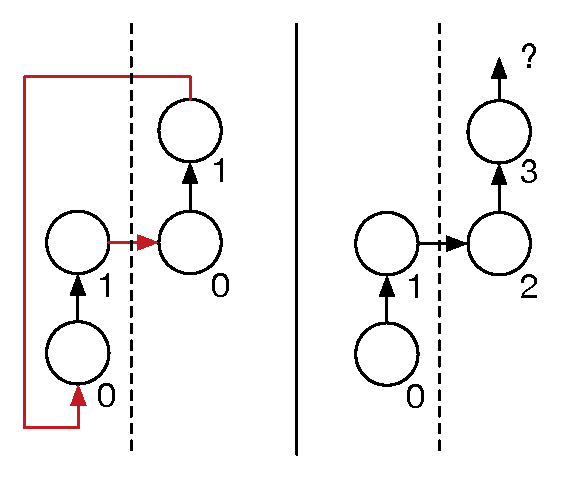
\includegraphics[]{5validation/images/cycle-prevention.pdf}
		\caption{CAPTION.}
		\label{fig:validation:cycle-prevention}
	\end{figure}
	
	\section{Consistent Cheating}
	\todo[inline]{Søren: Up until now, and I fear it will continue,
		chapter 5 has been quite hard to
		follow. As a reader you get the
		impression that I'm just plowing the
		web a rise of definitions that has, yes,
		something to do with DCR graphs and
		executing histories, but the exact
		connection is not clear to me, nor
		where we're going. I think you might
		need a bit more text helping the reader
		along the way, with comments like "We
		now look at the problem of ... We saw
		this with timestamps, which help}
	Until now we have examined inconsistent cheating, but malicious events are also able to cheat consistently:
	\begin{definition}
		\textbf{Consistent cheating} is the act of manipulating data in a way where the history is still valid.
		\textbf{Consistent cheating} is the act of participating in the creation of histories which are incorrect but valid.
	\end{definition}
	
	\newpar Consistent cheating can take a number of forms:

	\newpar \textbf{Incorrect timestamps}: A malicious event manipulates the timestamps of the actions in the history, while still being in accordance to Lamport's logical clocks
	\figuretodo{to historikker der er ens bortset fra timestamps}
	The only actions which more that one event know of are the action which are part of a relation. The consequence of this is that it is only possible to check if events disagree on the timestamps of these actions and not the rest. To make this validation each ingoing action is matched with outgoing actions and if it is not possible to find a match, one of the events must be malicious. 
	
	\newpar \textbf{Incorrect number of executions}: The history of a malicious event states that it has executed either fewer or more times than it has done.
	\figuretodo{to historikker hvor antallet af executions ikke matcher}
	To check for this kind of cheating each pair of events that have relations are examined. If event A and event B is examined, then the amount of every outgoing action from A to B must match the amount of ingoing actions on B from A. If the amount does not match then one of the events must be malicious and vice versa.
	
	\newpar \textbf{Incorrect number of incoming actions}: The history of a malicious event states that it has been affected either fewer or more times than what has happened.
	\figuretodo{to historikker hvor antallet af incoming groups ikke matcher }
	This type of cheating is already checked for by the method introduced in the previous paragraph.
	
	\newpar To argue there are no more ways to consistently cheat it is necessary to examine what possible activities an event can take part of. An event can execute or it can be affected by an execution. Not executing is just as valid as doing so (if the state of the workflow allows it). Furthermore, an action with a timestamp which is in accordance to Lamport's logical clocks, can have another timestamp which is also in accordance and therefore it is not possible to distinguish the correct timestamp from the incorrect. \todo[inline]{this paragraph has bullshit argumentation of the types being complete. plz help it}
	
	\subsection{Cases}
	Detecting and identifying consistently cheating events is difficult, because it is not possible to look at a single event's history and determine if it is valid or not. We will now examine how the structure of the DCR graph, and the connection between malicious events contribute to the ability to detect and identifying consistent cheating. The type of relation has no influence on the cases and relations are therefore visualised as a simple arrow from event to event.
	
	\newpar \textbf{Case 1 - Single Malicious Event}: In this case (see \ref{fig:consensus:single-malicious}), the event does not share relations with any other event, there is no one to disagree with any timestamps on actions and, in addition, completely oppose to the fact that an execution has happened or not. Therefore in workflows or subworkflows that include such events, it is not possible to identify or even observe if any kind of consistent cheating has happened.
	
	\begin{figure}[H]
		\centering
		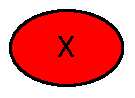
\includegraphics[]{5validation/images/1.pdf}
		\caption{}
		\label{fig:consensus:single-malicious}
	\end{figure}
	
	
	\newpar \textbf{Case 2 - Single Malicious Event With Relation to Self}: This case (see \ref{fig:consensus:single-malicious-with-relation}), just like case 1, in this case there are no one but the event itself to disrupt the cheating and therefore it is not possible to observe or identify consistent cheating.
	
	\begin{figure}[H]
		\centering
		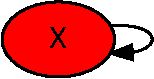
\includegraphics[]{5validation/images/5.pdf}
		\caption{}
		\label{fig:consensus:single-malicious-with-relation}
	\end{figure}
	
	\newpar \textbf{Case 3 - Single Malicious Event With Relation to Good Event}: In this case (see \ref{fig:consensus:single-malicious-with-good-relation}), the malicious event has a relation to a correctly working event. If the malicious event tries to cheat by changing the timestamps, it can do so in two ways. It can try to change the timestamps of the actions corresponding to the relation with the correctly working event, but in that case the two events will not agree on what happened and we are able to observe that one of them must cheat. Due to the fact that any of the two events could be malicious and change the timestamps it would not be possible to identify which of the two are evil.
	If the timestamp changes are on action which not related to the good event then it is not possible to observe nor identify. 
	\figuretodo{figur eksempler til tekst, der viser hvordan at to events kan være uenige}
	In the same way when looking at more or fewer executions, the relation action in the executions should have a counterpart but might not have. In the scenario where there are fewer executions the correctly working event will have actions with no counterpart and therefore it is only possible to observe and not identify this kind of cheating. 
	
	\begin{figure}[H]
		\centering
		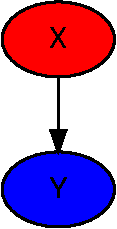
\includegraphics[]{5validation/images/3.pdf}
		\caption{}
		\label{fig:consensus:single-malicious-with-good-relation}
	\end{figure}
	
	\newpar \textbf{Case 4 - Single Good Event With Relation to Single Malicious Event}: In this case (see \ref{fig:consensus:single-good-with-malicious-relation}), a good event has a relation to a malicious event. Similarly to case 3 timestamp changes are observable due to the same factors, but instead of disagreeing on the outgoing relation in this case the malicious event will disagree on whether the good event executed or not. Due to the fact that when the malicious event executes the good event will not have any information about it, because it is not affected by that execution, the malicious event is able change the number of executions to its liking.
	\figuretodo{figur helt ens til den overfor men nu med den anden historik ond}
	 
	\begin{figure}[H]
		\centering
		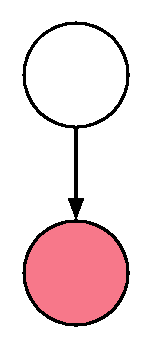
\includegraphics[]{5validation/images/2.pdf}
		\caption{}
		\label{fig:consensus:single-good-with-malicious-relation}
	\end{figure}
	
	\newpar \textbf{Case 5 - Single Good and Single Malicious Event with Relations to each other}: In this case (see \ref{fig:consensus:single-good-with-twoway-malicious-relation}), the situation is similar to that of case 3 and 4 in the sense that it provides the same ability to observe and the cheater.
	
	\begin{figure}[H]
		\centering
		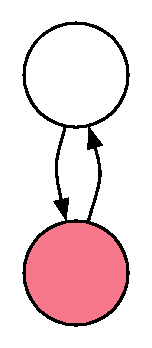
\includegraphics[]{5validation/images/6.pdf}
		\caption{}
		\label{fig:consensus:single-good-with-twoway-malicious-relation}
	\end{figure}
	
	\newpar \textbf{Case 6 - Single Malicious Event A with relation to Single Malicious Event B}: In this case (see \ref{fig:consensus:single-malicious-with-twoway-malicious-relation}), two malicious events work in collaboration to manipulate the data. Because a malicious event is also unpredictable, one of the events could function as a correctly functioning event and create the same depicting scenarios as in case 3 and 4, any absence of manipulation actually corresponds to the event functioning correctly.
	
	If it is assumed that both events work in collaboration to manipulate the history, it is both possible to change timestamps in such a way that it is not observable if they agree on the numbers, or observable if they disagree. Furthermore fewer or more executions is equally easily obscured if they agree on it.
	
	\figuretodo{figur: eksempel på hvordan de kan tilføje flere executions sammen}
	
	\begin{figure}[H]
		\centering
		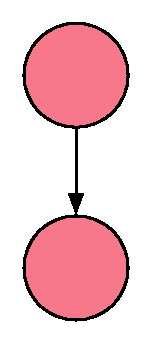
\includegraphics[]{5validation/images/4.pdf}
		\caption{}
		\label{fig:consensus:single-malicious-with-twoway-malicious-relation}
	\end{figure}
	
	\newpar \textbf{Case 7 - Two Malicious Events With Relations To Eachother}: In this case (see \ref{fig:consensus:two-malicious-with-twoway-malicious-relation}), two malicious events work in collaboration with to manipulate data with both their relations. This situation has the same properties as case 6.
	
	\begin{figure}[H]
		\centering
		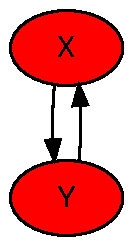
\includegraphics[]{5validation/images/7.pdf}
		\caption{}
		\label{fig:consensus:two-malicious-with-twoway-malicious-relation}
	\end{figure}
	
	\newpar In none of these cases had the property of being able to identify which of the events are malicious (in case 1 and 2 it is not possible to observe and therefore neither to identify), which creates some interesting questions as to how one can try to identify which of the events are cheating. One method could be to determine by counting how many of the neighbouring events disagree with you and if a majority disagrees the event will be marked as evil. Unfortunately that method has pitfalls since a good event with connection only to evil events could be marked as malicious. If we require a new property of the DCR graph which states that in all neighbourhoods with $N$ events, a maximum of $N/2-1$ are malicious an election would not be able to falsely accuse a good event of being malicious. This property is commonly used for distributed systems which uses elections, but traditionally is only used to describe the amount of malicious nodes in the entire system. Therefore this property is more strict and perhaps more difficult to adhere to. To worsen the situation substantially even if this property is adhered to, if an event is malicious does not mean that it is always malicious meaning it would be able to trick an election into not having a majority against it, so it is not possible to say that each event which disagrees with the values are malicious, which places us in the same situation as to begin with where we can only say one of two events must be malicious.
	
	\newpar It becomes apparent that the structure of the DCR graph has a great influence on whether it is possible to observe consistent cheating or not - especially in cases where a lot of malicious events create interconnected or not connected to any other event at all it can be difficult to say anything about the state of the history. One could argue what implications consistent cheating have on sub-graphs such as those of case 1 and 2, since their these events have little consequences on the rest of the workflow state and these events can only exist in two states (before and after they are executed) and therefore not being able to handle these kinds of situations is not that big a flaw. The true problems clearly happen in situation 6 and 7 where for example a company can own a sub part of the graph with many events working together to create a falsified image of what has happened. 
	
	\newpar Therefore a highly interconnected DCR graph is preferred if the users want to have a high probability of observing 

    \subsection{Simulation}\label{sec:historyindcr:simulation}
    One of the more difficult validity properties to check is whether events only executed when the state of the workflow allowed it. To do so, a lot of challenges must be addressed, it is not enough to check if the initial state of the event is executable, its, conditions also need to be taken into perspective, furthermore the state of the workflow possibly changes over time with each execution. In addition since the history is a strictly partially ordered set some executions happen concurrently which does not match physical time in which the events hav executed in.
    
    \newpar An approach to this problem is to simulate the executions of the workflow. To do so, it is required that the rules of the workflow and the initial state of every event in the workflow is known. Furthermore it is required that an order of execution has been found, this is examined in the next chapter but we assume it is available. 
    
    Given the order of execution each execution has either zero or more ingoing edges. Each ingoing edge states which executions must have happened before, therefore an execution can first happen when all of its ingoing edges have executed. Therefore each execution have a counter based on the amount of ingoing edges which can be decreased each time one of the ingoing edges executes. An order of execution based on a valid history will always have some executions which have no ingoing edges since no cycles appear and some events must happen before all their relations. 
    
    \newpar To check if an execution was possible, first it is checked if the the state of the corresponding event is executable. Then the state of every condition the event has are checked for being either excluded or executed. If the event was executable, the state of the workflow is changed according to the rules of the workflow. Then for every outgoing edge in the order of execution the counter is reduced by one. 
    
    \newpar To simulate the entire order of execution, the executions are checked for their ability to execute in a topological order. The order is created based on the counter value, where lower values are taken first. The order of which executions have happened are adhered to, but concurrent executions happen in a random order.
    
    Executions can only be concurrent if the events they belong to do not share outgoing relations. If two events share outgoing relations, one of them must affect the shared event before the other and an order would be able to be created. Therefore in an order of execution only one of the ingoing edges can be of an ingoing relation, the rest must be based on outgoing relations which can determine that the execution happens after some other executionn. The order of which concurrent executions are simulate therefore does not matter since they order of which they execute can only result in one state change which affects common outgoing edges.
    
    \newpar If an execution was not executable, it is possible to identify if it is the event itself which is malicious or if it is one or more of the condition events. If the state of the event was not executable then the event must be malicious, note that the conditions in this case also could be malicious. If the state is executable and the conditions are included and not executed, another situation arises. The conditions could have returned false information to the executing event, or the executing event could have executed regardless of the values returned. Therefore in this case only a set of possible malicious events can be determined.

	\newpar On \todo{create and ref} the algorithm can be seen. It runs in linear time to the amount of nodes
	
	\figuretodo{figur over en order of executions med counters på hver executions - eventuelt en ekstra med hvordan det ser ud efter at x events har executed}
	
	\begin{algorithm}[H]
		\begin{algorithmic}
			\Function{UpdateState}{state, event, relationType}
				\State locals: DCR rules
				\State (included, pending, executed) $\leftarrow$ \Call{Map.Get}{event, state}
				\If{relationType is SetsPending}
					\State \Call{Map.AddOrUpdate}{event, (included, true, executed), state}
				\ElsIf{relationType is Includes}
					\State \Call{Map.AddOrUpdate}{event, (true, pending, executed), state}
				\ElsIf{relationType is Excludes}
					\State \Call{Map.AddOrUpdate}{event, (false, pending, executed), state}
				\EndIf
				\State \Return state
			\EndFunction
			
			\State
			
			\Function{IsExecutable}{state, conditions, execution}
				\If{not \Call{Map.Get}{event, state}.Included}
					\Return false
				\EndIf
				\ForAll{event e, in conditions}
					\State localState $leftarrow$ \Call{Map.Get}{event, state}
					\If{not localState.included OR not localState.executed}
						\Return false
					\EndIf
				\EndFor
				\Return true
			\EndFunction
			
			\State
			
			\Function{Execute}{state, DCRRules, execution}
				\State conditions $leftarrow$ \Call{List.Where}{id == execution.Id and is conditionType, DCRRules}
				\State relations $leftarrow$ \Call{List.Where}{id == execution.Id and not is conditionType, DCRRules}
				\State state' $leftarrow$ \Call{UpdateState}{state, execution, r}
				\ForAll{event e, relation r in relations}
					\State state $leftarrow$ \Call{UpdateState}{state, e, r}
				\EndFor
				\If{\Call{IsExecutable}{state, conditions, execution}}
					\Return Success state'
				\ElsIf
					\Return Failure state' 
				\EndIf
			\EndFunction
			
			\State
			
			\Function{Simulation}{Graph, DCRRules, state}
			\State orderedExecutions $\leftarrow$ \Call{Graph.TopilogicalSort}{Graph} \Comment Returns a queue
			\State failures $\leftarrow$ List.Empty
			\While{not orderedExecutions.isEmpty}
				\State execution $\leftarrow$ \Call{Queue.Pop}{orderedExecutions}
				\State executeResult $\leftarrow$ \Call{Execute}{state, DCRRules, execution}
				\If{executeResult.IsFailure}
					\State failures $leftarrow$ \Call{List.Add}{execution, failures}
				\EndIf
				\State state $leftarrow$ execute.ResultState
				\State counterMap $leftarrow$ \Call{UpdateCounterMap}{execution, counterMap}
			\EndWhile
			\Return failures
			\EndFunction
			
			
		\end{algorithmic}
		\caption{Simulation algorithm}
		\label{alg:simulation}
	\end{algorithm}
	\todo{Check lige op på hvorfor vi tjekker executability efter det er vi opdaterer state i execute metoden}
	
	\newpar This algorithm is based on the forward chaining algorithm of entailment in propositional theorem proving\todo{ref section 7.5 in SISP bog}, which also runs in linear time and is used to see if a knowledge base can entail a proposition. 
	
    \newpar There is a couple of challenges and approaches to how it is handled both if cheating has been observed before the simulation or cheating is observed during the simulation. We have chosen the approach to mark if an execution was inconsistent, but allow it to "execute" and then change the state to see if the rest of the order of execution was consistent. One could easily check the rest of the order of execution without the state change of the inconsistent execution to see what implications that cheating could have had.